% Chapter 5
\newenvironment{my_desc}
{\begin{description}
  \setlength{\itemsep}{0cm}
  \setlength{\parskip}{0cm}}
{\end{description}}

\chapter{Software Design Description (SDD)} % Main chapter title

\label{Chapter5} % For referencing the chapter elsewhere, use \ref{Chapter5} 

\lhead{Chapter 5. \emph{Classifier Features}} % This is for the header on each page - perhaps a shortened title

\section{Introduction}
In Chapter 4, the project conceptualization was introduced as well as the proposed workflow and business requirements.

In this chapter, system architecture, main components and their functionalities, and how different components interact are to be discussed in section 5.3 . In section 5.4, the module interface for each component will be introduced.
%----------------------------------------------------------------------------------------
\section{Overview}

\subsection{Purpose}
This chapter shows how the smart email software system will be structured to satisfy the requirements identified in the conceptual design document and software requirements specification. It is a translation of requirements into a description of the software
structure, software components, interfaces, and data necessary for the implementation phase.

\subsection{Scope}
Smart email will provide automated email classification and foldering service for email clients. This chapter describes how the system will be divided into modules and the design details for each module.

\subsection{Definitions and acronyms}
  \begin{my_desc}
    \item[SDD] Software Design Description
    \item[TBD] To Be Defined
    \item[IMAP] Internet message access protocol
    \item[WEKA] Collection of machine learning algorithms for solving data mining problems implemented in Java and open sourced under the GPL.
    \item[MOA] Massive Online Analysis (MOA) is a software environment for implementing algorithms and running experiments for online learning from evolving data streams.
  \end{my_desc}


\section{References}
  \begin{my_desc}
\item[IEEE]  IEEE Std. 1016-1998 IEEE Recommended Practice for Software Design 
Description.
\item[D. Delaney] ``Document Templates For Student Projects in Software Engineering''
National University of Irelan, 2002
  \end{my_desc}

\section{Decomposition description}
This project is designed using an incremental approach. There are two primary  stages to the design development which consists of Phase 1 (Classification Module) and Phase 2 (Web Service Module).

The classification module can be divided into three layers. The data layer will be 
responsible for retrieving emails from file systems or using IMAP protocol. The 
second layer is the preprocessing and email filtering layer. This layer is 
responsible for filtering emails and extracting classification features from the 
email. The third and last layer will be responsible for classifying emails and 
testing the classifier performance.

The detailed design for each design entity is illustrated in the detailed class 
diagram at the end of this chapter.

\subsection{System decomposition}
The system is divided into main modules as follows:
\begin{my_itemize}
\item Classification Module;
\item Web Service Moudle.
\end{my_itemize}
Each of these modules will be described in details in the upcoming subsections.

\subsubsection{Classification Module}

\begin{my_itemize}
  \item ClassificationManager class
  \begin{my_desc}
    \item[Purpose] Used to manage and control the classification process flow
      with the dataset and classification algorithms.
    \item[Functions] TBD
  \end{my_desc}
  \item PreprocessingManager class
  \begin{my_desc}
    \item[Purpose] Used to manage preprocessing phase by applying selected data preprocessors
      to given raw emails.
    \item[Functions] \hfill
    \begin{my_itemize}
      \item apply(email:Email) used to apply the selected preprocessors on a given email.
    \end{my_itemize}
  \end{my_desc}

  \item FilterManager class
  \begin{my_desc}
    \item[Purpose] Used to manage feature extraction phase from preprocessed emails by applying
      specified set of filters.
    \item[Functions] \hfill
    \begin{my_itemize}
      \item getInstances(emails:List$\langle$Email$\rangle$) given a set of emails returns a prepared dataset (Instances object)
      \item getInstance(email:Email) given an email return a prepared feature vector (Instance object)
    \end{my_itemize}

  \end{my_desc}

  \item FilterCreatorManager class
  \begin{my_desc}
    \item[Purpose] Used to manage all Filter creators to create specified filters given a list of emails
    \item[Functions] \hfill
    \begin{my_itemize}
      \item getFilters(emails:List$\langle$Email$\rangle$) create all supported filters using given emails
    \end{my_itemize}

  \end{my_desc}


  \item Instances class
  \begin{my_desc}
    \item[Purpose] Used to gather all instances of the emails and treated as the classifier
      dataset.
    \item[Fuctions] \hfill
    \begin{my_itemize}
      \item add(instance:Instance) add new instance to the dataset.
      \item getAttribute(index:int) get Attribute at given index.
      \item getAttribute(name:String) get Attribute with the given name.
      \item checkInstance(instance:Instance) check if the given instance is in the dataset or not.
      \item getClassAttribute() return the class attribute of the dataset.
    \end{my_itemize}

  \end{my_desc}

  \item Instance class
  \begin{my_desc}
    \item[Purpose] Used to encapsulate the feature vector of a certain email.
    \item[Functions] \hfill
    \begin{my_itemize}
      \item getClassIndex() returns the index of the class attribute
      \item setClassIndex(index:int) set the index of the class attribute
      \item isMissingClass() check if the feature vector contains value of the class attribute or not
      \item getValue(index:int) return the value for the ith attribute
    \end{my_itemize}

  \end{my_desc}

  \item Attribute class
  \begin{my_desc}
    \item[Purpose] Used to encapsulate the dataset attribute with its type
    \item[Functions] \hfill
    \begin{my_itemize}
      \item Attribute(name:String) \\
      used to create a new Attribute instance with the given name.
      \item Attribute(name:String,nominals:ArrayList$\langle$String$\rangle$) \\
      used to create a new Attribute instance with the given name and possible values.
      \item getValue(int:index): String \\
      returns the attribute possible value of the given index
      \item getIndexofValue(value:String): int \\
      returns the index of the given attribute possible value
    \end{my_itemize}

  \end{my_desc}

\end{my_itemize}

\subsubsection{Web Service Module}
The web service module will be responsible for providing the clients with ability to classify their emails. The web service will be supported for Gmail mail servers as a first step. The detailed design for this module will be complemeted before the expected start date for this phase (The first of April).

\subsection{Data decomposition}
The data layer is responsible for retrieving emails either from the file system or using the IMAP protocol. The enron data set will be used as the data source for training and testing the email classifier.

\subsubsection{Data access object}
  \begin{my_desc}
   \item[Purpose] This class is responsible for retrieving emails using the IMAP protocol.
   \item[Function] This class inherits from the data access object class.
  \end{my_desc}

\subsubsection{IMAP data access object}
  \begin{my_desc}
   \item[Purpose] This class is responsible for retrieving emails using the IMAP protocol.
   \item[Function] This class inherits from the data access object class.
  \end{my_desc}


\subsubsection{File system data access object}
  \begin{my_desc}
   \item[Purpose] This class is responsible for retrieve emails from the file system.
   \item[Function] This class inherits from the data access object class.
  \end{my_desc}


\section{Interface description}
The interface description provides everything designers, programmers and testers need to know to correctly use the functions provided by the system entities. This description includes the details of external and internal interfaces not provided in the software requirements specification.

\subsection{Module interface}
\subsubsection{Classification module interface}
\begin{my_itemize}
  \item Classifier class
  \begin{my_desc}
   \item[Purpose] All schemes for documents classification extend this class. Note that a classifier MUST either implement distributionForInstance() or classifyInstance() methods.
   \item[Function] The Classifier abstarct class defines the following functions:
	\begin{my_itemize}
		\item classifyInstance(Instance instance) : classifies a given instance;
		\item buildClassifier(Instances trainingData) : builds the classification model from the given set of training data;
		\item getClassifierByName(String name, String[] options) : returns an instance of the classifier given the classifier name;
		\item distributionForInstance(Instance instance): returns the destribution for each class attribute for the given instance.
	\end{my_itemize}
  \end{my_desc}

  \item Preprocessor interface
  \begin{my_desc}
   \item[Purpose] Performs some pre-processing actions on the email before classifiaction. Pre-processing may include removing stop words and stemming. 
   \item[Function] The Preprocessor interface defines the following function:
	\begin{my_itemize}
	\item process(Email email): Performs some pre-processing action on the given email such as stemming or removing stop words.
	\end{my_itemize}
  \end{my_desc}

  \item Filter class
  \begin{my_desc}
   \item[Purpose] Defines an abstract class for filtering an email. A filter is used to extract a set of features from the email such as the email sender, email label and word frequencies in an email.
   \item[Function] The filter abstract class defines the following set of functions:
	\begin{my_itemize}
	\item makeFeatureInstance(Email email): creates a feature instance from the given email.
	\item getAttributes(): returns the set of attributes for the given filter.
	\end{my_itemize}
  \end{my_desc}

  \item FilterCreator interface
  \begin{my_desc}
   \item[Purpose] Defines an interface for creating a filter.
   \item[Function] The FilterCreator interface defines the following function:
	\begin{my_itemize}
	\item createFilter(emails:List$\langle$Email$\rangle$): creates a filter given the list of emails.
	\end{my_itemize}
  \end{my_desc}

\end{my_itemize}

\subsubsection{Web service moudle interface}
TBD

\section{Detailed design}

\subsection{Classification module detailed design}

\begin{figure}
  \centering
  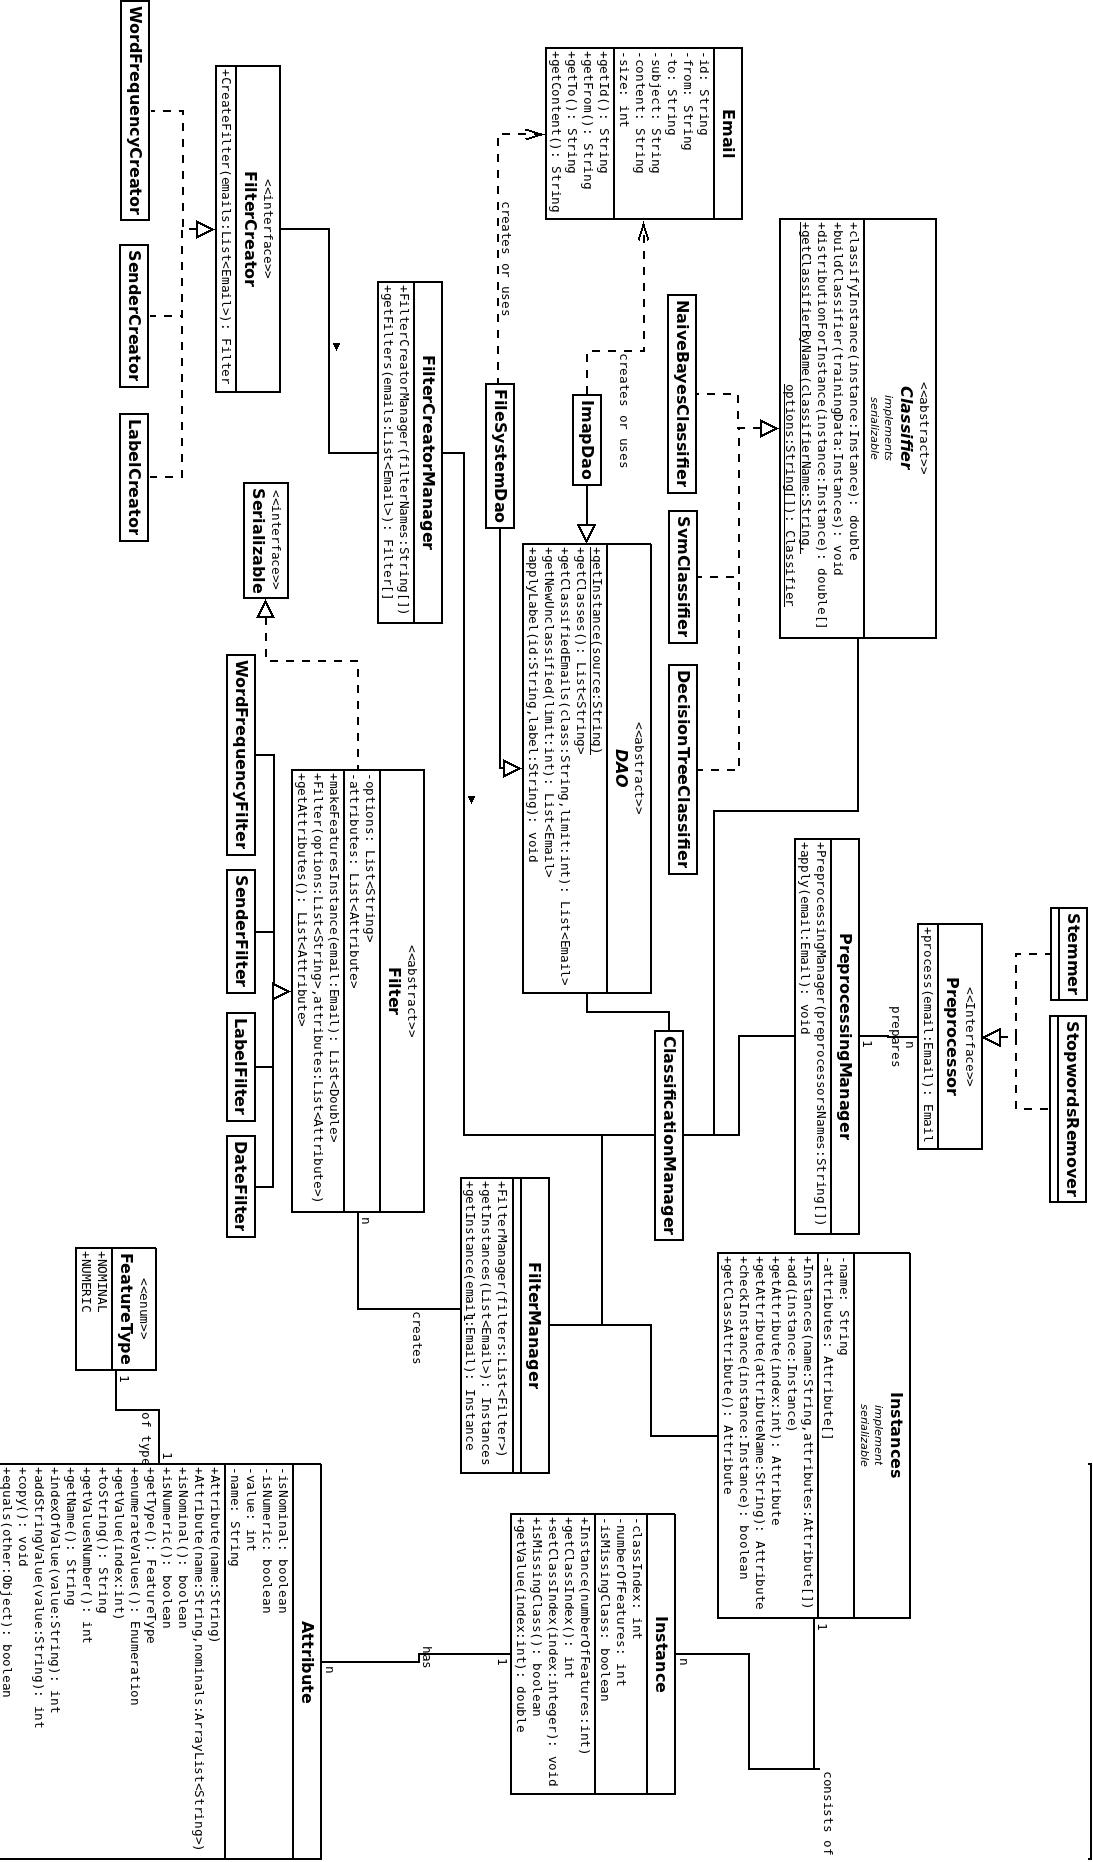
\includegraphics[width=12cm]{design.jpeg}
  \caption[Detailed Design] {Detailed Design}
\end{figure}




\subsection{Web service module detailed design}
TBD

\section{Conclusion}
In this chapter, the system architecture was introduced and the abstract system design using was illustrated.

In the next chapter, the performance evaluation for the email classifier will be discussed.
